\section{Stationary stochastic process}

\begin{definition}[\textit{Stationary stochastic process}]
    A stationary stochastic process (in a wide sense) is a stochastic process characterized by the following properties:
    \begin{itemize}
        \item The mean must be constant: 
            \[m(t)=m\qquad\forall t\]
        \item The covariance is dependent solely on $\tau=t_2-t_1$: 
            \[\gamma(t_1,t_2)=\gamma(t_2-t_1)=\gamma(\tau)\]
    \end{itemize}
\end{definition}

The properties of this function are:
\begin{enumerate}
    \item The variance is non-negative: 
        \[\gamma(0)=\mathbb{E}\left[{\left(v(t)-m\right)}^2\right]\geq 0\]
    \item The covariance is less or less or equal than the variance: 
        \[\left\lvert \gamma(\tau) \right\rvert \leq \gamma(0) \qquad \forall\tau\]
    \item The function is even: 
        \[\gamma(\tau)=\gamma(-\tau) \qquad\forall\tau\]
\end{enumerate}

\begin{property}
    Given a stationary stochastic process $v(t,s)$, we denote its mean and covariance function as $m_v$ and $\gamma_v(\tau)$, respectively.
\end{property}
\begin{property}
    Two stationary stochastic processes $v_1(t,s)$ and $v_2(t,s)$ are wide-sense equivalent if $m_{v_1}=m_{v_2}$ and $\gamma_{v_1}(\tau)=\gamma_{v_2}(\tau)$ for all $\tau$.
\end{property}
\begin{definition}[\textit{Correlation function}]
    The correlation function is defined as: 
    \[\mathbb{E}\left[ v(t,s)v(t-\tau,s) \right]\]
\end{definition}


\begin{example}
    Consider the process $v(t,s)=\alpha(s)$, where $\alpha(s) \sim \mathcal{N}(1,3)$. 
    \begin{figure}[H]
        \centering
        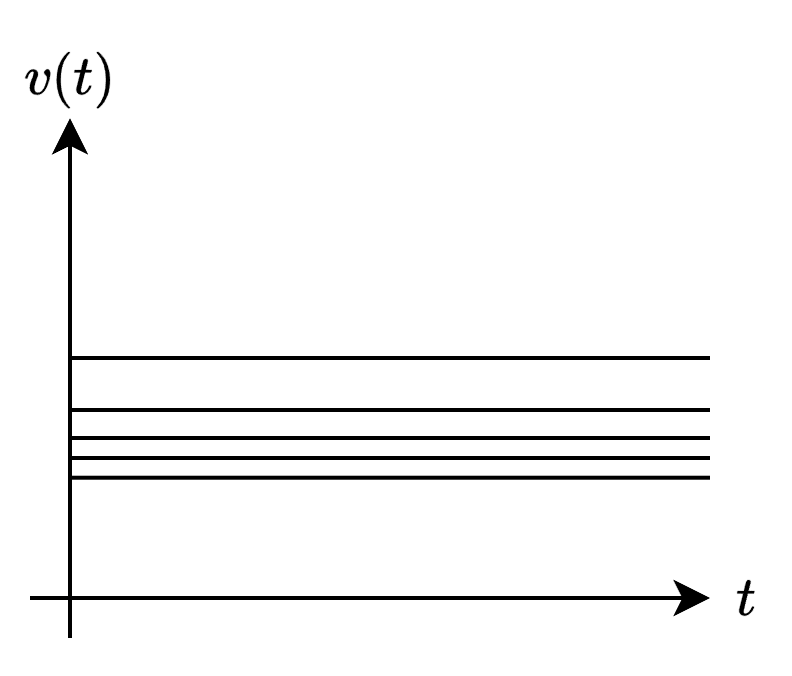
\includegraphics[width=0.35\linewidth]{images/static.png}
        \caption{Some possible realizations}
    \end{figure}
    All the realizations are constants and are more frequent near the value one.

    To determine if this is a stationary stochastic process, we need to verify: 
    \begin{enumerate}
        \item Constant mean: 
            \[m(t)=\mathbb{E}\left[v(t,s)\right]=1\]
        \item The covariance must be a function of only $\tau$: 
            \begin{align*}
                \gamma(t,t-\tau)&=\mathbb{E}\left[\left(v(t,s)-m(t)\right)\left(v(t-\tau,s)-m(t)\right)\right] \\
                                &=\mathbb{E}\left[\left(\alpha(s)-1\right)\left(\alpha(s)-1\right)\right] \\
                                &=3
            \end{align*}
    \end{enumerate}
    Both functions are $t$-invariant, thus the process is weakly stationary.
\end{example}

\begin{example}
    Consider the process $v(t,s)=t\alpha(s)-t$, where $\alpha(s) \sim \mathcal{N}(1,3)$. 
    \begin{figure}[H]
        \centering
        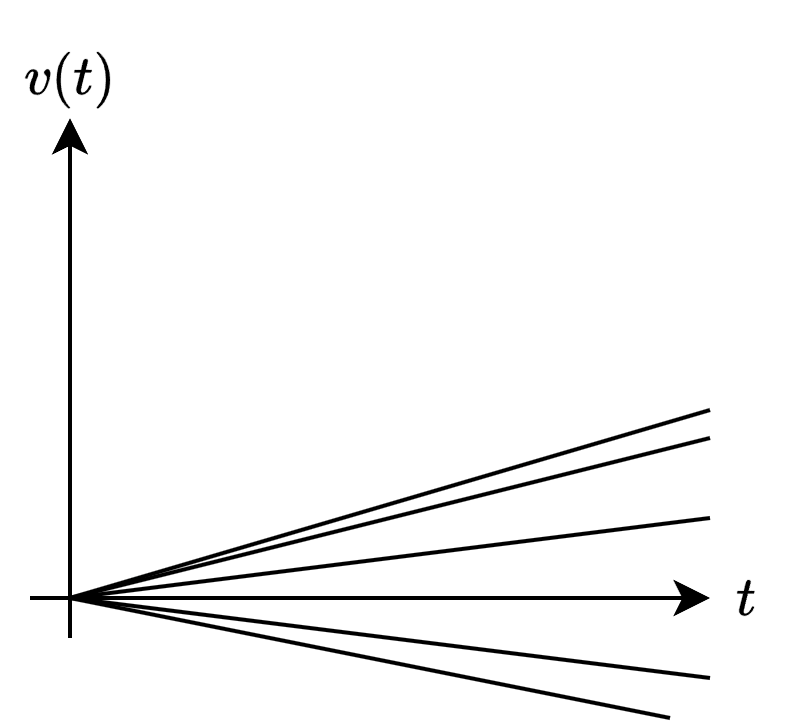
\includegraphics[width=0.35\linewidth]{images/stationary.png}
        \caption{Some possible realizations}
    \end{figure}
    All the realizations are not constants, but they are more frequent near the value one.
    
    To determine if this is a stationary stochastic process, we need to verify: 
    \begin{enumerate}
        \item Constant mean: 
            \[m(t)=\mathbb{E}\left[v(t,s)\right]=\mathbb{E}\left[t\alpha(s)-t\right]= t\mathbb{E}\left[\alpha(s)\right]-t =t-t=0\]
        \item The covariance must be a function of only $\tau$: 
            \begin{align*}
                \gamma(t,t-\tau)&=\mathbb{E}\left[\left(v(t,s)-m(t)\right)\left(v(t-\tau,s)-m(t)\right)\right] \\
                                &=\mathbb{E}\left[\left(t\alpha(s)-t-m(t)\right)\left((t-\tau)\alpha(s)-(t-\tau)-m(t)\right)\right] \\
                                &=\mathbb{E}\left[\left(t\alpha(s)-t\right)\left((t-\tau)\alpha(s)-(t-\tau)\right)\right] \\
                                &=\mathbb{E}\left[t\left(\alpha(s)-1\right)(t-\tau)\left(\alpha(s)-1\right)\right] \\
                                &=(t^2-t\tau)\mathbb{E}\left[{\left(\alpha(s)-1\right)}^2\right] \\
                                &=3(t^2-t\tau)
            \end{align*}
    \end{enumerate}
    The covariance function is $t$-variant, thus the process is not weakly stationary.
\end{example}